\documentclass{sig-alternate-05-2015}
  \pdfpagewidth=8.5truein
  \pdfpageheight=11truein
  
  \usepackage{graphicx}
  \usepackage[portuguese, english]{babel}
  \graphicspath{ {images/} }
  \usepackage[utf8]{inputenc}
  \usepackage[justification=centering]{caption}
  \usepackage{amsmath}
  \usepackage{multirow}
  \usepackage{makecell}
  \usepackage{cite}
  \usepackage{booktabs}
  %\usepackage{changes}
  \usepackage[final]{changes}
  \usepackage{enumerate}
%  \usepackage{subfigure}
\usepackage{caption}
\usepackage{subcaption}

\begin{document}

\hyphenation{semi-au-to-mat-ic}

% Copyright
\setcopyright{acmcopyright}
%\setcopyright{acmlicensed}
%\setcopyright{rightsretained}
%\setcopyright{usgov}
%\setcopyright{usgovmixed}
%\setcopyright{cagov}
%\setcopyright{cagovmixed}

% DOI
\doi{http://dx.doi.org/xx.xxxx/xxxxxxx.xxxxxxx}

% ISBN
\isbn{978-1-4503-3739-7/16/04}

%Conference
%\conferenceinfo{PLDI '13}{June 16--19, 2013, Seattle, WA, USA}

\acmPrice{\$15.00}

%
% --- Author Metadata here ---
\conferenceinfo{SAC'16,}{ April 4-8, 2016, Pisa, Italy}
\CopyrightYear{2016} % Allows default copyright year (20XX) to be over-ridden - IF NEED BE.
%\crdata{0-12345-67-8/90/01}  % Allows default copyright data (0-89791-88-6/97/05) to be over-ridden - IF NEED BE.
% --- End of Author Metadata ---

\title{Exploring the Combination of Software Visualization and Data Clustering in the Software Architecture Recovery Process}


\numberofauthors{1} %  in this sample file, there are a *total*
% of EIGHT authors. SIX appear on the 'first-page' (for formatting
% reasons) and the remaining two appear in the \additionalauthors section.
%
%\author{
% You can go ahead and credit any number of authors here,
% e.g. one 'row of three' or two rows (consisting of one row of three
% and a second row of one, two or three).
%ah
% The command \alignauthor (no curly braces needed) should
% precede each author name, affiliation/snail-mail address and
% e-mail address. Additionally, tag each line of
% affiliation/address with \affaddr, and tag the
% e-mail address with \email.
%
% 1st. author
%\alignauthor
%Renato Paiva, Genaína N. Rodrigues,  Rodrigo Bonif\'{a}cio\\
%      \affaddr{Computer Science Department}\\
%     \affaddr{University of Brasília}\\
%    \affaddr{Brasilia, Brazil}\\
%    \email{\{renatoedesio}@unb.br\},\\
%   \{genaina, rbonifacio\}@cic.unb.br}



\maketitle
\begin{abstract}
Modernizing a legacy system is a costly process that requires deep understanding of the system architecture and its components. Without an understanding of the software architecture that will be rewritten, the entire process of reengineering can fail. \deleted{When there is absence of architectural documents, it is important to have a recovery process of architecture that allows the complete understanding of the software. Such process involves mapping of source code entities in high-level models.} \replaced{For this reason, semi-automatic and automatic techniques for architecture recovery have been active focuses of research. However, there are still important improvements that need to be addressed on this field of research w.r.t achieving a more accurate architecture recovery process.}{Previous work using visualization and clustering techniques has been proposed and extensively used. However, their accuracy to reconstruct the architecture alone has shown to be not satisfactory enough.} In this work, we propose to explore if an approach where visualization and clustering applied together can provide a higher accuracy on the software architecture recovery process. An experimental study was conducted in a industrial environment to empirically evaluate our investigation. Our results indicated a statistically significant increase in the accuracy of the recovery process.
\end{abstract}


%
% The code below should be generated by the tool at
% http://dl.acm.org/ccs.cfm
% Please copy and paste the code instead of the example below. 
%
\begin{CCSXML}
<ccs2012>
 <concept>
  <concept_id>10010520.10010553.10010562</concept_id>
  <concept_desc>Computer systems organization~Embedded systems</concept_desc>
  <concept_significance>500</concept_significance>
 </concept>
 <concept>
  <concept_id>10010520.10010575.10010755</concept_id>
  <concept_desc>Computer systems organization~Redundancy</concept_desc>
  <concept_significance>300</concept_significance>
 </concept>
 <concept>
  <concept_id>10010520.10010553.10010554</concept_id>
  <concept_desc>Computer systems organization~Robotics</concept_desc>
  <concept_significance>100</concept_significance>
 </concept>
 <concept>
  <concept_id>10003033.10003083.10003095</concept_id>
  <concept_desc>Networks~Network reliability</concept_desc>
  <concept_significance>100</concept_significance>
 </concept>
</ccs2012>  
\end{CCSXML}

\ccsdesc[500]{Computer systems organization~Embedded systems}
\ccsdesc[300]{Computer systems organization~Redundancy}
\ccsdesc{Computer systems organization~Robotics}
\ccsdesc[100]{Networks~Network reliability}


%
% End generated code
%

%
%  Use this command to print the description
%
%\printccsdesc

% We no longer use \terms command
%\terms{Theory}

\keywords{Software Architecture Recovery; Software Visualization; Data Clustering}

\section{Introduction}

Software modernization in an activity that requires a significant understanding 
of the architecture. Nevertheless, this is a challenge because usually there is a 
lack of architecture information and thus some reverse engineering practices 
must take place. Moreover, the ability to mine relevant information from 
execution traces tend to quickly become large and unmanageable and, for this reason, 
it is necessary to filter part of those traces and extract relevant information 
for the particular understanding of the task being performed \cite{canfora_achievements_2011}. 
In most cases, understanding the software structure is also a challenging task due to the lack of 
architecture specification documents, particularly w.r.t legacy systems.  
If there is no such specification available or if it is out-of-date, a software architecture recovery 
process must take place.
%The required effort to manually recover a system architecture is proportional to the the size and complexity of its source code. 
%This is particular more costly for large software systems, prone to every sort of errors \cite{zapalowski_revealing_2014}. 
As a result, the study of methods and tools to extract the software systems architecture is fundamental to guarantee a faster and more accurate process. 
%By these means, costs and risks in the process of architecture recovery should be diminished.

Software visualization is a widely used technique for architecture recovering~\cite{ghanam_survey_2008, teyseyre_overview_2009, lanza_codecrawler-lessons_2003, Feijs_loe}. 
\added{They are \emph{semi-automatic} techniques that reconstruct the software architecture by manually abstracting low-level knowledge, 
due to interactive and expressive visualization tools \cite{ducasse_software_2009}.} The basis of the software visualization underlies 
on the creation of a representation of the system via visual elements~\cite{teyseyre_overview_2009}. 
Using such abstraction, it is possible to obtain a new view of the software, which allows exploring different concepts and 
clearer understanding of the software system structure.

Despite the improvement on the results obtained through \replaced{semi-automatic techniques}{software visualization techniques}, most of the times, 
the efficiency of the methods or tools rely on the ability of the analyst in charge of the software architecture recovery. As a result, the accuracy of the results,\added{particularly 
to derive the modular decomposition of the software}, is bound by subjective criteria most of the times. In order to fill in this gap, 
various research work has been devoted to automate the architecture recovery process. For instance, \added{software clusterization 
is an automatic technique} to recover a software system architecture\cite{shtern_clustering_2012, Jain_Murty_1999, Wiggerts, mitchell_heuristic_2002}. 
%\added{This technique assists software architects to identify groups of objects (such as a modular 
%decomposition of a system) whose members are similar in some way \cite{ducasse_software_2009}}.  
%Such technique is used in various fields 
%of research to describe methods to cluster unclassified data.  
In the context of architecture recovery, clustering techiniques aims at grouping software artifacts in significant modules, leading towards an understanding of 
the software system structure in a higher abstraction level \cite{shtern_clustering_2012}.

However, although both approaches for architecture recovering have been widely discussed in the literature, 
there is no empirical study that investigates how each technique complements each other. 
In this paper we 
carried out an experiment that aims at understanding how the combination of both approaches improve 
the accuracy of the models obtained from an architectural recovery. The contributions of the paper 
are two fold 

\begin{itemize}
\item It presents the design, execution, and main findings of an empirical study that 
investigates the benefits of combining well-known semi-automatic visualization and clustering 
techniques for architecture recovering. 

\item It reports that the combination of the selected approaches improves the accuracy of the 
resulting models--- that improvement ranges from 19\% to 30\%, depending on 
the visualization and programming language techinique we used in our experiment.   

\end{itemize}

% However, to decompose a software system in higher-level structures in a coherent and logic coupling, 
% is an inherently difficult task.  Due to the usual sparse set of data in a source code and the various 
% computational factors involved in a software system, many solutions are only suboptimal and do not represent 
% the real software architecture \cite {mitchell_heuristic_2002}.  On the other hand, results of such technique are 
% still helpful as they provide as a result a view of the software system decomposition, instead of reconstructing it from scratch. 
% Further refinements are then required in order to have an accurate architecture recovery \cite{tzerpos_comprehension-driven_2001}.

%Given the inaccuracy inherent to architecture recovery techniques, one question comes out:  Is it possible to obtain a more accurate software architecture recovery process? 
%We propose to investigate this question by merging both \replaced{quasi-manual and quasi-automatic techniques}{visualization and clustering techniques} into one  architecture 
%recovery process. We postulate that  \replaced{quasi-manual and quasi-automatic techniques, such as software visualization and clustering, respectively,} {clustering and visualization  techniques} 
%are complementary in the sense that they provide different levels of software architecture abstraction. Our investigation is performed on a controlled 
%experiment in a industrial environment, where participants are software analysts and developers working on software systems developed in Java and Visual Basic programming languages. 
%Our results show a statistically significant improvement in the accuracy of the models produced from our proposal compared to the techniques used alone.

The remaining sections of the paper are structured as follows: Section 2 presents related work regarding software architecture visualization and clustering techniques. Section 3 highlights the inaccuracies of such techniques and the principles that drive our investigation. Section 4 is the main section where we present and evaluate the experimental study we conducted with the software development group in the Data Processing Center at University of Brasilia. In Section 6 we conclude our work and present the future directions we plan to pursue.


\section{RELATED WORK}\label{sec:related}

\deleted{Maintenance and evolution of software systems is an expensive and challenging task. For this reason, several approaches for the recovery of software architecture have been proposed. Ducasse et al. in \cite{ducasse_software_2009} present a taxonomy of approaches to architecture recovery, detailing information necessary for recovery, such as: what the stakeholders’ goals are, how the general reconstruction proceeds, what the available sources of information are. Based on this, which techniques one can apply and what kind of knowledge the process provides.} In this section we report most recent work that leveraged the discussion comparing accuracy and effectiveness of recovery techniques.

Garcia \textit{et al.} \cite{Garcia:ASE2013} performed a comparative analysis of six automated architecture recovery techniques. The selected techniques rely on two kinds of input obtained from im\-ple\-mentation-level artifacts: textual and structural. The accuracy of the techniques were assessed on eight architectures from six different open-source systems. Their results indicated that two of the selected recovery techniques are superior to the rest along multiple measures. However, the results also show that there is significant room for improvement in all of the studied techniques, particularly w.r.t accuracy.

Lutellier \textit{et al.} \cite{Lutellier_2015} compared nine variants of six architecture recovery techniques using two different types of dependencies: symbol and include. Four of the selected techniques use dependencies to determine clusters, while the remaining two techniques use textual information from source code. The results shows that symbol dependencies generally produce architectures with higher accuracies than include dependencies. Despite this improvement, the overall accuracy is low for all recovery techniques.

Regarding the context of semi-automatic techniques, Wettel \textit{et al.} \cite{wettel_software_2011} carried out a controlled experiment to investigate the efficacy and effectiveness of the CodeCity software visualization tool in the process of understanding a software system structure. Results pointed out that analysis via CodeCity was possible to obtain an accuracy of 24.26\% and a reduction of 12.01\% in the execution time of a certain number of tasks, when compared to an understanding process carried out manually. %inspection of the source code.
\section{RATIONALE ON THE COMBINATION BETWEEN VISUALIZATION AND DATA CLUSTERING}\label{sec:rationale}%

In many cases, the analyst, with some knowledge of a system, can perform an analysis of the results and create a concise final model. However, especially for complex systems, it is necessary to use strategies to correctly interpret the results. Such strategies involve the observation of repeated patterns and identification of architectural violations in the source code.

In general, automatic architecture reconstruction methods, such as clustering techniques, have the advantage to produce different models for a single software system in a short period of time. Such models can be constructed differently by changing configuration settings on clustering algorithm used during the process. Through the analysis of different models it is possible to identify patterns that recur frequently in the results. One of the most prominent software clustering tool is Bunch~\cite{mitchell_heuristic_2002}, which transforms the architecture recovery problem into an optimization problem. Bunch uses hill-climbing and genetic algorithms to find the software cluster partitions that maximizes the modularization quality.  Bunch provides the Nearest Ascent Hill Climbing (NAHC) as default.

However, when the idea is not clear of how the system structure is composed, the various models produced by clustering process may not suffice to understand the complex software \cite{craft}, since the results show a high level view of the architecture. In this sense, the use of software visualization techniques allow a fine-grained observation of different outcomes on a low level of abstraction. By means of interactive operations in the models produced by the visualization software, it is possible to decompose components of the system in more detailed representations. Thus, allowing the observation of concepts as part of the architecture in greater depth.

In this context, linking the models produced by the clustering process with the model produced by the software visualization process, it is possible to get different representations of the system to form a final model with greater precision. For example, take into account the results shown in Figure \ref{exemplo_comparacao_modelos}. Assuming that the process of obtaining architecture models recovered four different results, through the use of software visualization technique and clustering algorithms. Each model features 9 entities, namely: \{1,2,3,4,5,6,7,8,9\}. By performing a count of the grouped entities it is  possible to obtain the ratio of how many times the entity was classified similarly to the other. The result of this count is observed in Table \ref{ocorrencias_1}.

\begin{table}[h]
	\centering
	\caption{Occurrences of entities in the results.}
	\label{ocorrencias_1}
	\begin{tabular}{|cc|}
		\hline
		\multicolumn{1}{|l}{Relation} & \multicolumn{1}{l|}{Occurrence} \\ \hline
		\{1,2,3\},\{7,8,9\}                  & 100\%                           \\ \hline
		\{4,5\}, \{6,7,8,9\}                    & 50\%                          \\ \hline
		\{1,2,3,4\},\{4,5,6\},\{5\},\{6\}                  & 25\%           \\ \hline
	\end{tabular}
\end{table}

By analyzing the results, it is possible to see that the entities \{1,2,3\} can be classified into a single module, since they appear 100\% of the times in the same relation; so do the entities \{7,8,9\}. The entities \{4,5,6\} may be classified as either a single module or each entity may be added to any other adjacent module, since there is no agreement between the results. In these cases, additional analysis must be performed for each entity. This simple example illustrates how to use different results to help the composition of a single final model. In many cases, the aggregation of results provide technical assistance, by highlighting the common patterns. It is possible to gain confidence that agreement across a collection of results can reflect the system structure \cite {craft}.

\begin{figure}[!h]
	\centering
	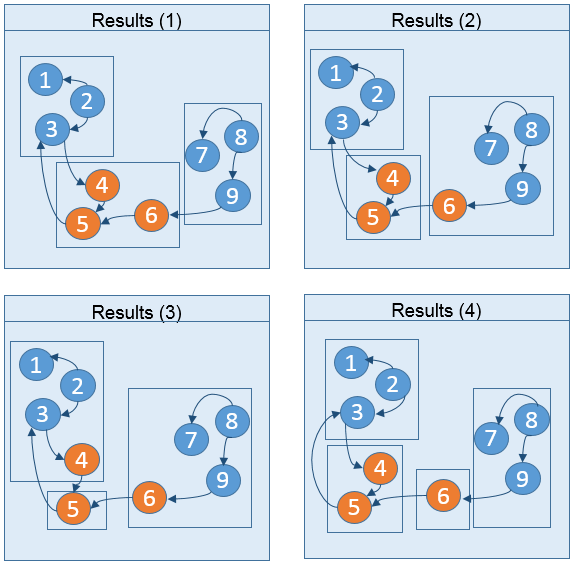
\includegraphics[width=0.3\textwidth]{exemplo_comparacao_modelos_en}
	\caption{Different results for comparison.}
	\label{exemplo_comparacao_modelos}
\end{figure}


However, a more careful analysis of the results, may reveal that other factors may influence the final model produced by clustering and visualization software techniques. A software system throughout its life cycle is susceptible to several changes in its architecture. However, such operations can introduce architectural violations in the code, for example, violation of the layers,  break of abstractions, feature duplication \cite {kazman_view_1998}. In this context, reverse engineering methods are strongly affected by those shortcomings in the system code base \cite {Platenius_2012}.  Such violations should be identified and addressed, so it does not affect the correctness of the final model.

To illustrate a violation on an architecture,  we will use the same results of Figure \ref{exemplo_comparacao_modelos}.  This Figure illustrates a representation of an architecture components through a dependency structure matrix. The figures depicts how the interaction works. The software elements are numbered from 1 to 4, where, for example, the Presentation module (2) requires information from the Visualization module (1). On the other hand, the figures shows also that the Visualization module (1) provides information to the Data module (4).

 \begin{figure}[!h]
 	\centering
 	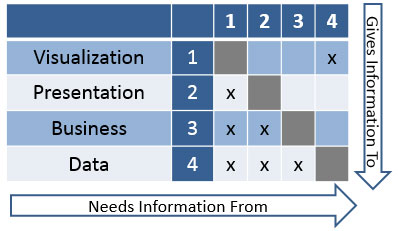
\includegraphics[width=0.3\textwidth]{3_exemploMatrizViolada_en}
 	\caption{DSM representation	of dependences.}
 	\label{3_exemploMatrizViolada}
 \end{figure}
 
 Assuming the entity 4 is wrongly mapped as part of a module. This happens due to a coupling between entities 4 and 5, which illustrates an architecture violation. All results would be classified differently if such violation was removed.\deleted{, as shown in Figure \ref{exemplo_comparacao_modelos2}}. The results of the new analysis, taking into account the aggregation of similar entities, can be seen in Table \ref{ocorrencias_2}. Analyzing the results, it is possible to check the impact of the violation. The module containing the first mapping \{1,2,3\} now adds  entity 4, since this set was rated similarly on all results. As for the mapping \{5,6\} there is also a higher chance of being classified in a same module, as it occurs with higher frequency.


\begin{table}[]
	\centering
	\caption{Occurrences of entities between the results after elimination of architectural violation}
	\label{ocorrencias_2}
	\begin{tabular}{|ll|}
		\hline
		\multicolumn{1}{|l}{Relation} & \multicolumn{1}{l|}{Occurrence} \\ \hline
		\{1,2,3,4\}, \{7,8,9\}  	 & 100\%                           \\ \hline
		\{5\}, \{5,6\}	& 50\%                            \\ \hline
		\{6\}, \{6,7,8,9\}	& 25\%                            \\ 
		\hline
	\end{tabular}
\end{table}

%\begin{figure}[!h]
%	\centering
%	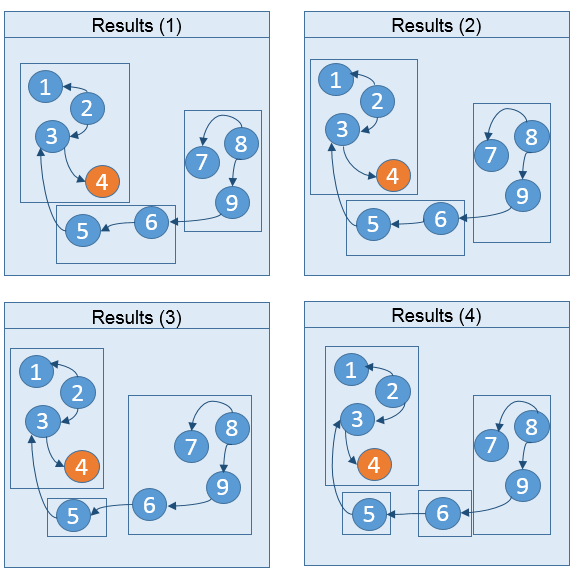
\includegraphics[width=0.43\textwidth]{exemplo_comparacao_modelos_2_en}
%	\caption{Eliminating the architectural violation of results.}
%	\label{exemplo_comparacao_modelos2}
%\end{figure}

Such violations can be found through an analysis of the artifacts produced by software visualization. As an example, take into account the dependency structure matrix shown previously in Figure \ref{3_exemploMatrizViolada}. Through observation of the DSM, it is possible to note a relationship exists between layers, and each layer depends on the upper layers. However, this relationship is violated by layer "Date" (4), since it uses resources of the layer  "View" (1), characterizing an architectural violation. Once the violation is detected, it should be treated as failure and, if necessary, modify the data set for the clustering process, so that the relationship is not considered. Thus, avoiding the production of wrong models that may affect the interpretation of the results.

\section{EXPERIMENTAL STUDY}\label{sec:experiment}

\added{The empirical} \deleted{Empirical} research presented in this work \deleted{experimental} aims to evaluate the combination
of well-known semi-automatic (software visualization) and automatic (software clustering) techniques in the context of a software architecture recovery to understand the modular decomposition of a system. \replaced{We guided our study}{The study was performed} using the Goal Question Metric (GQM) approach, as described in Table~\ref{tab:RecoveryTechniques}.
\begin{table}[!h]
	\centering
	\caption{Definition of the accuracy evaluation Software Architecture Recovery Techniques.}
	\resizebox{\columnwidth}{!}{%
	\begin{tabular}{@{}ll@{}}
		\toprule
		\textbf{Purpose}   & Evaluate    \\
		\textbf{Issue}     & architecture recovery accuracy\\
		\textbf{Object}    & semi-automatic \& automatic techniques\\
		\textbf{Viewpoint} & software architect \& application engineer\\
		\textbf{Context}   & industrial environment
	\\ \bottomrule
	\end{tabular}
	}
	\label{tab:RecoveryTechniques}
\end{table}

The underlying research question for this experiment is as follows: 
\emph{Does the use of software visualization technique, along with the clustering technique, increase the accuracy of the architectural model produced, in comparison with using one of the techniques alone?}
  
\subsection{Design}%

%This section presents the experimental design of this research, in a level of details that might help other researchers to replicate our study~\cite{Juristo_2010} using a similar setting.

%% \deleted{This section describes the experiment plan 
%% and demonstrates how 
%% the experiment was designed. This allows the execution of 
%% other studies based on the same plan~\cite{Juristo_2010}.}

The study considered four software systems, written in two distinct programming languages (Visual Basic and Java). Table \ref{tabelaSistemasObjetos}  presents relevant information on the characteristics of each object of the experiment. Systems A 
and B are legacy systems still operating in the University of Brasilia, and both support the management of the academic routine of college students. Systems C and D have been developed on a new platform, in order to modernize legacy systems written in Visual Basic. These systems deal with administrative university routines.

\begin{table}[h]
	\centering
	\caption{Systems objects used in the experiment.}
	\label{tabelaSistemasObjetos}
	\begin{tabular}{|lllll|}
		\hline
		System  & Language    & LOC   &  methods & files  \\ \hline
		System A-Sae             & Visual Basic & 25425 & 1551       & 133        \\
		System B-Sigra           & Visual Basic & 36169 & 2828       & 218        \\
		System C-Siex            & Java         & 19609 & 2699       & 195        \\
		System D-SisRu           & Java         & 14238 & 1734       & 178        \\ \hline
	\end{tabular}
\end{table}

%\subsubsection{Subject selection}%

The participants involved in the experiment are system developers, with different levels of experience. We selected a total of ten participants \replaced{that agreed to voluntarily participate in the study}{using a convenience approach, that is, the participants volunteered for participating in the study}. Subjects were randomly divided into two groups, henceforth called Group 1 and Group 2. At the beginning of each session, participants were asked about their level of knowledge in relevant aspects related to architecture recovery. Figure~\ref{fig:participantes}(a) and Figure~\ref{fig:participantes}(b) detail the expertise of the participants in the first and second groups, respectively. The y-axis represents the percentage of professionals in the corresponding expertise level.

\begin{figure*}[htb]
 \begin{subfigure}{0.5\textwidth}
	\centering
	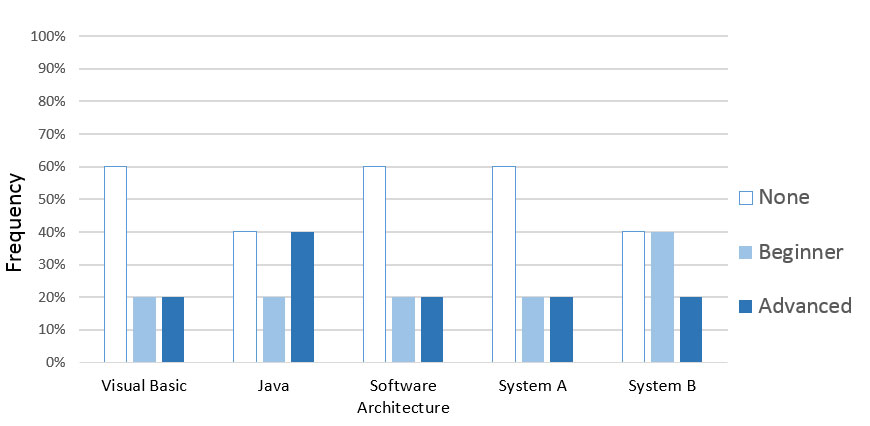
\includegraphics[scale=0.25]{6_expertise_participantes_grupo_1_en}
	\caption{Participants expertise in Group 1.}
%	\label{conhecimentoGrupo1}
 \end{subfigure}
 \begin{subfigure}{0.5\textwidth}
	\centering
	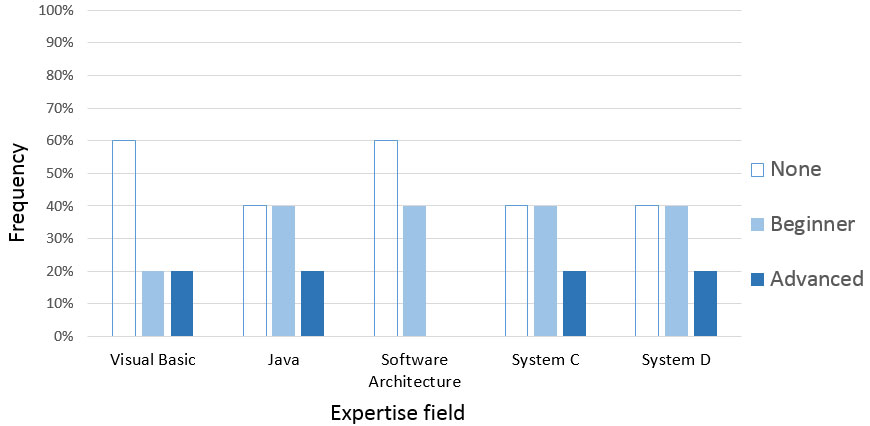
\includegraphics[scale=0.25]{6_expertise_participantes_grupo_2_en}
	\caption{Participants expertise in Group 2.}
 \end{subfigure}
\caption{Expertise of the participants.}
\label{fig:participantes}
\end{figure*}

%Figure \ref{conhecimentoGrupo2} details information about the level of knowledge of 
%participants in Group 2.

%% \begin{figure}[!h]
%% 	\centering
%% 	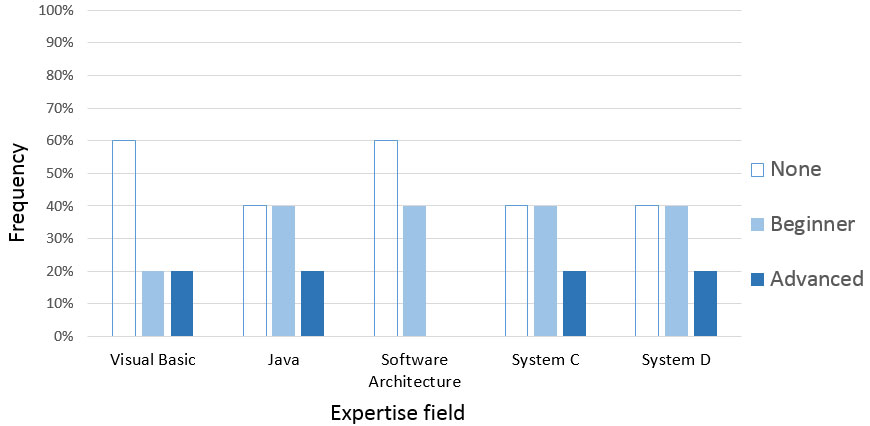
\includegraphics[width=0.45\textwidth]{6_expertise_participantes_grupo_2_en}
%% 	\caption{Participants expertise in Group 2.}
%% 	\label{conhecimentoGrupo2}
%% \end{figure*}

\added[remark={seria importante descrever quais s\~{a}o 
as vari\'{a}veis envolvidas, e quais fatores precisam / est\~{a}o 
sendo controlados com esse design. como os grupos foram formados? 
talvez uma leitura do artigo SoSyM ajude.}]

%% \begin{figure}[!h]
%% 	\centering
%% 	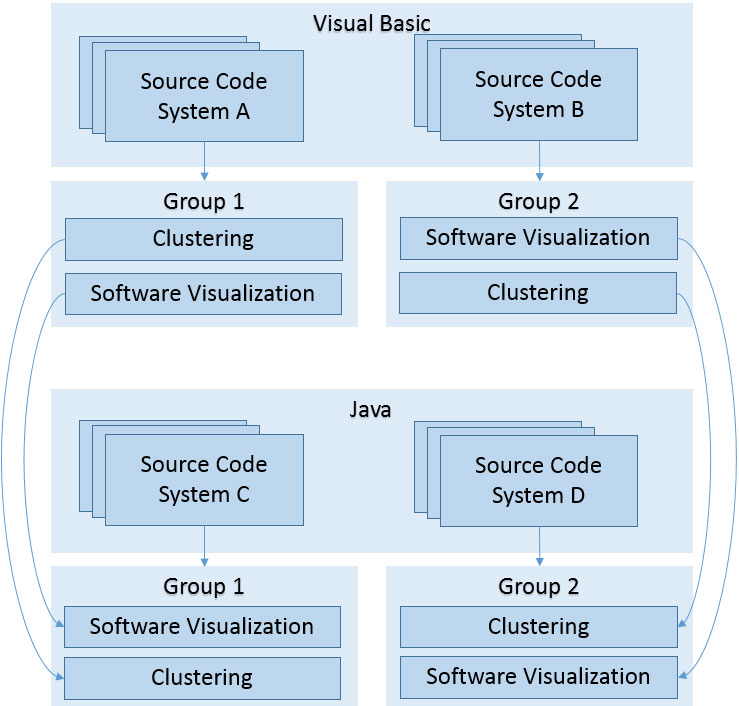
\includegraphics[width=0.43\textwidth]{design_experimento}
%% 	\caption{Design of the experiment.}
%% 	\label{design_experimento}
%% \end{figure}


{\subsection{Execution}%
\replaced{In order to level the knowledge of the participants, basic architecture concepts were introduced for each participant, as well as the essential elements for detecting the overall architecture of the object systems.}{Architecture recovery is an interpretive and interactive process involving many activities. Therefore, it may be a time consuming task. For this reason, the experiment seeks to recover the overall modular decomposition of the systems architecture. So, for each participant, the basic architecture concepts were introduced, as well as the essential elements for detecting the overall architecture of the object systems. The semi-automatic analysis of the Visual Basic system was carried out using the \texttt{VBDepend} tool. This tool provides several mechanisms that facilitates the exploitation of the system architecture in Visual Basic language based on visualization via dependency graphs and dependency structure matrix. Figure \ref{matrizDependenciaVBDependend} highlights a dependency structured  matrix (DSM)~\cite{Tekinerdogan_2009} obtained using \texttt{VBDepend} 
tool. }

% TODO: talvez levar esse texo para a secao de background.

% In this case, the DSM is useful for analyzing the properties of complex applications. 
% In an architectural analysis, the couplings between the architectural modules are described and various operations on the matrix can be performed in order to identify architectural relations \cite{Tekinerdogan_2009}.

\deleted{\begin{figure}[!h]
	\centering
	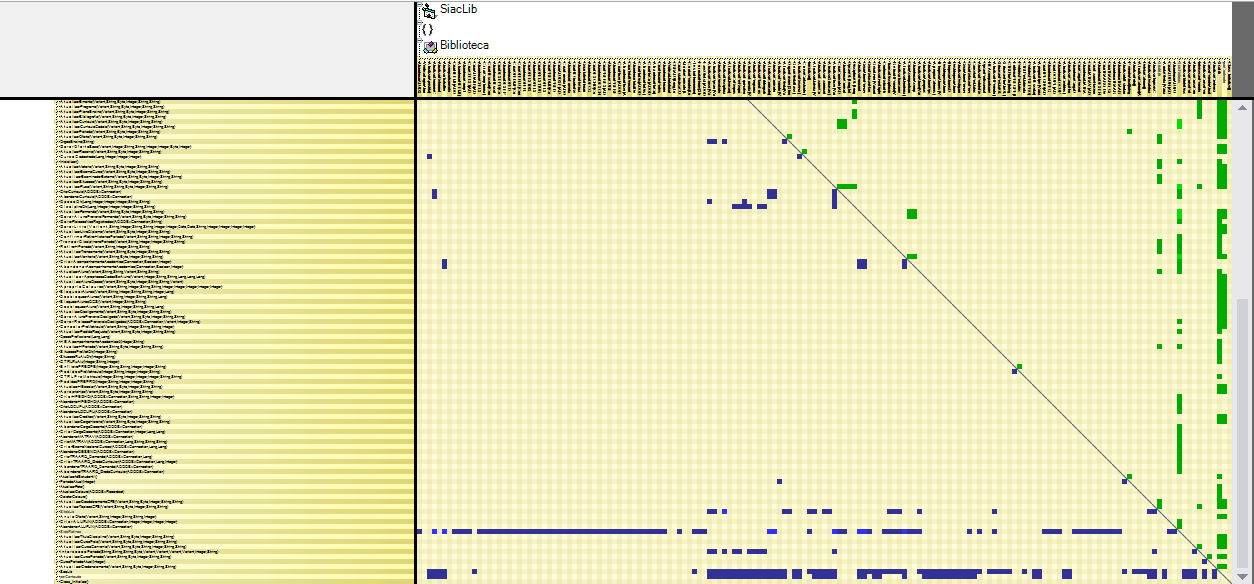
\includegraphics[width=0.45\textwidth]{6_matrizDependenciaVBDependend}
	\caption{Dependency matrix obtained through the use of VBDepend tool.}
	\label{matrizDependenciaVBDependend}
\end{figure}}

\replaced{The semi-automatic analysis of the Visual Basic system was carried out using the \texttt{VBDepend} tool~\cite{VBDepend} ,which is based on visualization via dependency graphs and dependency structure matrix. While to analyse the Java systems, the subjects used two different tools: \texttt{ X-Ray} \cite{X-Ray} and \texttt{Architexa}  \cite{Architexa}. Both Java analysis tools are plug-ins for the Eclipse IDE. Through these tools, one can get different views of class-package dependencies and systemic complexity views on Java projects. The \texttt{Bunch} tool \cite{mitchell_heuristic_2002} was used for the automatic approach of the architecture recovery. Participants were instructed to use the default Nearest Ascent Hill-Climbing algorithm (NAHC) implemented in the tool.}{To analyse the Java systems, the subjects used two different tools: \texttt{X-Ray} and \texttt{Architexa}. The X-Ray software visualization tool is an open source software available as a plug-in for the Eclipse IDE. Through this tool, one can get different views of class-package dependencies and systemic complexity views on Java projects. An example of a systemic complexity view can be seen in \ref{xray_complexidade}. In this kind of view, classes are represented by rectangles; the width of the rectangles representing the number of methods implemented in a particular class, while the height of the rectangle represents the number of lines of code in the class. The bonding edge is the relationship between the classes. The nodes can be set as a vertical tree, highlighting the hierarchy of classes.}

\deleted{\begin{figure}[!h]
	\centering
	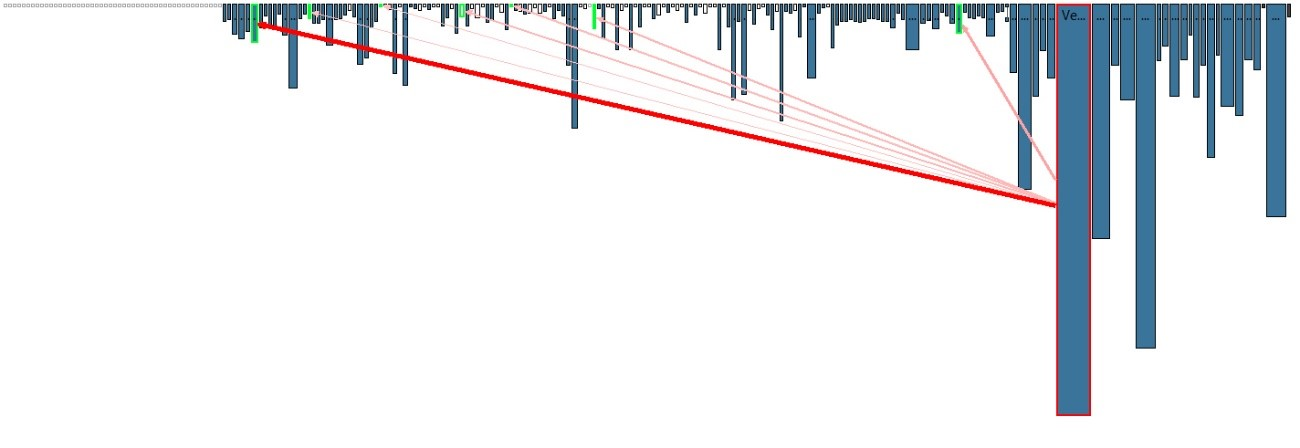
\includegraphics[width=0.45\textwidth]{6_xray_complexidade}
	\caption{Extracted systemic complexity view of a system in Java.}
	\label{xray_complexidade}
\end{figure}}

\deleted{Another tool used for viewing the source, and available to the participants of the 
experiment is the \texttt{Architexa}. With this tool it is possible to create 
different diagrams from the static analysis of the code. It is also available as a plug-in for 
the Eclipse IDE. Using this tool, the participants of the experiment can explore different 
aspects of the source code, such as a diagram of layers, as in Figure \ref{diagrama_architex}. The diagram layers groups classes based on their respective directories or packages and illustrates the dependency relationships between them. Also, different metrics can be used to highlight important aspects of the system, 
for example, the rectangle representing the software entities. Software entities that contain a large amount of code are represented by rectangles proportional to their size, which facilitates the identification of important aspects of the code structure. When selected a software entity, the visualization tool displays its respective dependencies by means of an arrow which indicates the origin and destination of the link. The 
thicker the arrow, the higher the correlation between the elements. Moreover, the colors of each rectangle are changed to emphasize the dependencies.}


\deleted{\begin{figure}[!h]
	\centering
	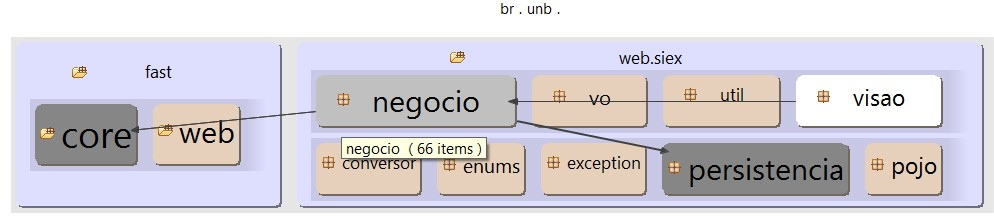
\includegraphics[width=0.45\textwidth]{6_diagrama_architex_2}
	\caption{Extracted systemic complexity view of a system in Java.}
	\label{diagrama_architex}
\end{figure}}


\deleted{The \texttt{Bunch} tool \cite{mitchell_heuristic_2002} was used as representant of the automatic approach for architecture recovery. It is an open-source initiative that implements a recovery approach based on clustering provides an intuitive graphical interface, as shown in {\color{red}Figure~\ref{}}. Participants in 
the experiment were instructed to choose between the available algorithms and run the clustering process in the system under analysis.
\added[remark={isso nao diminui o controle do experimento? isso nao diminui as chances de replicar o estudo?}]{The participants were able to change} the input 
parameters of the algorithms and run the clustering tool as often as they felt necessary. \texttt{Bunch} generates a file containing the modules automatically mapped from the selected algorithm. Through the output of the analysis, the participants comprised the architectural model of the system under analysis.}

%Participants in Group 1 started the extraction in a Visual Basic system using the clustering technique. The results of this extraction was collected. Then we presented the second technique (a semi-automatic visualization tool) and requested the subjects to produce a second model, applying both techniques. Afterwards, the same procedure was applied to the Java systems, but on the reverse order, i.e, first using a software visualization tool and then clustering. For the participants in Group 2, the same procedure applied, but starting with the software visualization technique.

For each of the two participating groups, we randomly selected one system in Java and one system in Visual Basic, so that in the end each group analyses systems in both languages. Then, each participant started the architecture recovery procedure by applying two reengineering approaches per session, which produced two models representing the modular decomposition of the system. In the first part of the session, the participant applied only one technique using either a semi-automatic decomposition based on software visualization or an automatic decomposition based on software clustering. After obtaining the first model, the other approach was presented and it was requested to produce a new model, based on the two techniques. We also made sure that the application order of each technique was prioritized in one of the two systems in each group. In this way, it was possible to calculate the accuracy of the resulting models using one technique, two techniques while varying their order of application.\footnote{The resulting models are available at https://github.com/ArchRecovery-SAC2016/files}.

To calculate the accuracy of the recovered architectural representation of the modular decomposition of the systems, and then answering the questions of the experiment, we used the Jaccard similarity coefficient, defined by the formula:

\begin{center}
	$Sj= \frac{a}{a+b+c}$
\end{center}

Here: $Sj$ is the coefficient of Jaccard; $a$= the number of common receovered 
modules; $b$= number of modules recovered in B but not in A; $c$= number of recovered modules in A, but not in B. In the experiment, model B was produced by a domain expert, while the model A was produced by \added{the} participants \replaced{of}{in} the experiment.

\subsection{Results}%

%Through the results, calculated from the comparison of the models produced by the participants with models produced by experts in the field, it was possible to investigate the use of architecture recovery approaches using a combination of automatic (clustering) and semi-automatic (software visualization) techniques to identify the modular decomposition of a system.  

To analyze the significance of the results, it was used the paired \texttt{t-test}. To use such parametric approach, we observed the different conditions that underpin the paired t-test, as: two related groups; no significant outliers; distribution of the differences in the dependent variable between the two related groups is approximately normally distributed. 

Table~\ref{tabelaResultadoVB} presents the comparison data between the scores obtained using one and two techniques. It is possible to realize that the average accuracy of the models obnained in Visual Basic sytems using one technique 
was approximately 51\%, and the average accuracy of the models obtained using the combination of both techniques was approximately 77\%--- that is, a difference of 26\%. 
On the other hand, it is possible to note that the mean of the models obtained in Java systems using one technique was approximately 48\%; when used both techniques, 
the mean was approximately 72\%--- a difference of almost 24\%.

\begin{table}[h]
	\centering
	\caption{Descriptive data table of the systems in Visual Basic and Java.}
	\label{tabelaResultadoVB}
	\resizebox{\columnwidth}{!}{%
	\begin{tabular}{|l|l|l|l|l|l|}
		\hline
		& Technique      & N  & Means & Std. Deviation & Std.Error Mean \\ \hline
		Visual Basic & One Technique  & 10 & 0.517 & 0.091          & 0.028          \\ \hline
		& Two Techniques & 10 & 0.771 & 0.077          & 0.024          \\ \hline
		Java         & One Technique  & 10 & 0.483 & 0.060          & 0.019          \\ \hline
		& Two Techniques & 10 & 0.728 & 0.059          & 0.018          \\ \hline
	\end{tabular}
	}
\end{table}

We also analysed whether these results are statistically meaningful, carring out the paired \texttt{t-test}. 
Table~\ref{tabelaResultadoTesteTVB} details the results of the test, comparing the results obtained using one technique 
with the outcomes obtained using two techniques (automatic and semi-automatic). To interpret the results it is necessary to observe the Sig. (2-tailed) value, also known as \texttt{p-value}. 

\begin{table}[h]
	\centering
	\caption{Paired t-test for Visual Basic systems.}
	\label{tabelaResultadoTesteTVB}
	\resizebox{\columnwidth}{!}{%
		\begin{tabular}{|l|l|c|c|c|c|l|l|l|}
			\hline
			& \multicolumn{5}{c|}{Paired  Diferences}                                                                                                                                                                                                             &                              &                         &                                                                                 \\ \cline{2-6}
			&                            & \multicolumn{1}{l|}{}                                    & \multicolumn{1}{l|}{}                                        & \multicolumn{2}{l|}{\begin{tabular}[c]{@{}l@{}}95\% Confidence \\ Interval\end{tabular}} &                              &                         &                                                                                 \\ \cline{5-6}
			& Mean                      & \begin{tabular}[c]{@{}c@{}}Std.\\ Deviation\end{tabular} & \begin{tabular}[c]{@{}c@{}}Std. Error\\ Mean\end{tabular} & Lower                                     & Upper                                     & \multicolumn{1}{c|}{t}       & \multicolumn{1}{c|}{df} & \multicolumn{1}{c|}{\begin{tabular}[c]{@{}c@{}}Sig. \\ (2-tailed)\end{tabular}} \\ \hline
			\begin{tabular}[c]{@{}l@{}}(Visual Basic) \\ One technique-\\ Two techniques \end{tabular} & \multicolumn{1}{c|}{-0.253} & 0.079                                                     & 0.025                                                         & -0.310                                        & -0.196                                        & \multicolumn{1}{c|}{-10.046} & \multicolumn{1}{c|}{9}  & \multicolumn{1}{c|}{0.000}                                                       \\ \hline
			
			\begin{tabular}[c]{@{}l@{}}(Java)\\One technique-\\ Two techniques\end{tabular} & \multicolumn{1}{c|}{-0.245} & 0.053                                                     & 0.0169                                                        & -0.283                                        & -0.207                                        & \multicolumn{1}{c|}{-10.046} & \multicolumn{1}{c|}{9}  & \multicolumn{1}{c|}{0.000}                                                       \\ \hline
				\end{tabular}
	}
\end{table}

Analyzing the data for the systems in Visual Basic, it is possible to conclude that there is a significant difference between the scores obtained using one technique ($Mean= 0.517$, $Std.\ Deviation = 0.091$) and two techniques ($Mean= 0.771$, $Std.\ Deviation= 0.077$); $t(9)=-10.046$, $p= 0.000$. So, with 95\% confidence, we can assume that there is an increase in results from 0.196 to 0.310 when used two techniques for software architecture recovery. Analyzing the data for the systems in Java language, it is possible to conclude that there is a significant difference between the mean values obtained using one technique ($Mean= 0.483$, $Std.\ Deviation= 0.060$) and two techniques ($Mean= 0.728$, $Std.\ Deviation= 0.059$); $t(9)= -10.046$, $p= 0.000$. Thus, with 95\% of confidence, the accuracy improvement varies from 0.207 to 0.283 when used two techniques for software architecture recovery. %For the sistems in Java

After these analyzes, it is possible to conclude that using two techniques produced better results than using only one technique in a software architecture recovery process. Thus, it is possible to answer our research question. 
%, where it is questioned whether the use of both techniques increases the accuracy of the obtained architectural models. 
Given the above results, we conclude that the use of both techniques significantly impacts the accuracy of the models produced, since all the results indicated an accuracy increase of the models when used the two techniques together.

%% \replaced{To enhance the results obtained, further analyzes were performed. First, }{To answer RQ2,}, we performed an analysis of the impact on the programming 
%% language on the accuracy of the results.  From Table \ref{tabelaOutrasAnalises2} it can be seen that in Visual Basic systems, the average accuracy of the models 
%% produced was approximately 60\%. In systems written in Java, the accuracy was approximately 64\%. These values represent the total amount of analyses performed for each language. 
%% Since each language was twice analysed in each group, then N equal 20, in this case.

%% \begin{table}[h]
%% 	\centering
%% 	\caption{Descriptive data table comparing system languages.}
%% 	\label{tabelaOutrasAnalises2}
%% 	\resizebox{\columnwidth}{!}{%
%% 	\begin{tabular}{|l|l|l|l|l|l|}
%% 		\hline
%% 		~         & Language      & N  & Mean   &  Std. Deviation   & Std. Error Mean \\ \hline
%% 		Pair1 & Visual Basic      & 20 & 0.605  & 0.138        & 0.031         \\
%% 		~         & Java           & 20 & 0.644  & 0.153        & 0.034         \\ \hline
%% 	\end{tabular}
%% 	}
%% \end{table}

%% To calculate the significance of the means difference and determine if the programming language affects the recovery process, we conducted a paired t-test. The result can be seen in Table \ref{table:test_t3}. Through data analysis, we conclude that there is no significant difference between the mean values of the systems in Visual Basic (Mean= 0.605,  Std. Deviation= 0.138) and Java systems (Mean= 0.644,  Std. Deviation= 0.153); t(19)= -1.867, p= 0.077. \replaced{Given the outcome,}{Thus it is possible to answer RQ2: given the outcome,} we can conclude that, with 95\% of confidence level, the programming languages had no statistically significant effect on the results, since Sig(2-tailed) value is greater than 0.05. So, the difference of means is in the interval (-0.082; 0.004), which includes 0.

%% \begin{table}[h]
%% 	\centering
%% 	\caption{Paired t-test for the comparison of the two programming languages.}
%% 	\label{table:test_t3}
%% 	\resizebox{\columnwidth}{!}{%
%% 		\begin{tabular}{|l|l|c|c|c|c|l|l|l|}
%% 			\hline
%% 			& \multicolumn{5}{c|}{Paired  Diferences}                                                                                                                                                                                                             &                              &                         &                                                                                 \\ \cline{2-6}
%% 			&                            & \multicolumn{1}{l|}{}                                    & \multicolumn{1}{l|}{}                                        & \multicolumn{2}{l|}{\begin{tabular}[c]{@{}l@{}}95\% Confidence \\ Interval\end{tabular}} &                              &                         &                                                                                 \\ \cline{5-6}
%% 			& Mean                      & \begin{tabular}[c]{@{}c@{}}Std.\\ Deviation\end{tabular} & \begin{tabular}[c]{@{}c@{}}Std. Error\\ Mean\end{tabular} & Lower                                     & Upper                                     & \multicolumn{1}{c|}{t}       & \multicolumn{1}{c|}{df} & \multicolumn{1}{c|}{\begin{tabular}[c]{@{}c@{}}Sig. \\ (2-tailed)\end{tabular}} \\ \hline
%% 			\begin{tabular}[c]{@{}l@{}}Visual Basic-\\ Java\end{tabular} & \multicolumn{1}{c|}{-0.0387} & 0.0928                                                     &  0.020                                                       & -0.082                                      & 0.004                                        & \multicolumn{1}{c|}{-1.867} & \multicolumn{1}{c|}{19}  & \multicolumn{1}{c|}{0.077}                                                       \\ \hline
%% 		\end{tabular}
%% 	}
%% \end{table}

We also analyzed if the order of the recovery technique affects the results. This analysis is useful to check whether starting from visualization or clustering in our process influences the accuracy of the results. Table~\ref{tabelaOutrasAnalises4} details the descriptive results of the data. When first using software visualization and then using clustering, the accuracy of the models obtained was approximately 77\%. Using first clustering followed by software visualization technique, the accuracy of the models 
obtained was approximately 72\%.

\begin{table}[h]
	\centering
	\caption{Descriptive data table related to the order of the techniques.}
	\label{tabelaOutrasAnalises4}
	\resizebox{\columnwidth}{!}{%
		\begin{tabular}{|l|l|l|l|l|l|}
			\hline
			 Order     						 & N  & Mean   & Std. Deviation   & Std. Error Mean  \\ \hline
			Visualization-Clustering  			  & 10  & 0.771  & 0.077        & 0.024         \\
			Clustering-Visualization          & 10  & 0.728  & 0.059        & 0.018         \\ \hline
		\end{tabular}
	}
\end{table}

To investigate the statistical significance of the difference between the means, it was conducted a paired \texttt{t-test}. The results are shown in Table \ref{table:test_t4}. Results show that, with  95\% confidence interval, the lower and upper limit range includes 0. As a result, it is possible to conclude that there is no statistical significance of the difference between the mean values obtained using software visualization prior to clustering or vice versa.

\begin{table}[h]
	\centering
	\caption{Paired t-test for the comparison of the order of techniques.}
	\label{table:test_t4}
	\resizebox{\columnwidth}{!}{%
		\begin{tabular}{|l|l|c|c|c|c|l|l|l|}
			\hline
			& \multicolumn{5}{c|}{Paired  Diferences}                                                                                                                                                                                                             &                              &                         &                                                                                 \\ \cline{2-6}
			&                            & \multicolumn{1}{l|}{}                                    & \multicolumn{1}{l|}{}                                        & \multicolumn{2}{l|}{\begin{tabular}[c]{@{}l@{}}95\% Confidence \\ Interval\end{tabular}} &                              &                         &                                                                                 \\ \cline{5-6}
			& Mean                      & \begin{tabular}[c]{@{}c@{}}Std.\\ Deviation\end{tabular} & \begin{tabular}[c]{@{}c@{}}Std. Error\\ Mean\end{tabular} & Lower                                     & Upper                                     & \multicolumn{1}{c|}{t}       & \multicolumn{1}{c|}{df} & \multicolumn{1}{c|}{\begin{tabular}[c]{@{}c@{}}Sig. \\ (2-tailed)\end{tabular}} \\ \hline
			\begin{tabular}[c]{@{}l@{}}VisualizationClustering-\\ ClusteringVisualization\end{tabular} & \multicolumn{1}{c|}{0.0427} & 0.0927                                                     &  0.029                                                       & -0.023                                      & 0.109                                        & \multicolumn{1}{c|}{1.456} & \multicolumn{1}{c|}{9}  & \multicolumn{1}{c|}{0.179}                                                       \\ \hline
		\end{tabular}
	}
\end{table}

% \deleted{Given the above, it is possible to answer RQ3, whether the order of the technique applied can affect the results.} 
% Facing the results, we can say that there is no statistical evidence to say that the order of the approach had an influence on the results, since Sig(2-tailed) value is greater than 0.05 resulting the interval (-0.023, 0.109) which includes 0.

\subsection{Discussion}

% The experimental study observed the impact of using data clustering and software visualization techniques in the understanding of software systems architecture.

% First, it was examined whether the use of software visualization and clustering techniques together improves the accuracy of the architecture recovery process. 

Altogether, the results showed that the accuracy of the models produced had a significant increase when two techniques were used together compared to using one technique alone, irrespective of the technique order applied. This suggests that the investigated techniques act in a complementary manner by providing additional information. Also, the use of both techniques together provided to the participants a different perspective of the software, not perceived or not represented when compared to using only a technique. 
%Thus, allowing for recovery of the architecture more accurately. 

%Second, an analysis was performed to verify if programming language can affect the recovery of the architecture. 
% The results showed that the programming language had no significant effect on the results. This demonstrates the 
% flexibility of clustering  and software visualization techniques. This flexibility is due to the fact that currently there are 
% several software visualization tools available, which enable the analysis of different programming languages. Also, the 
% clustering approach, implemented by Bunch tool, is designed to be independent of language, since it is only necessary 
% to set up a MDG containing the dependency relationships between the entities of the source code, and this is achieved through static analysis techniques of the source code.

In addition, we observed that the order of execution of the techniques does not significantly affect the results. This indicates that there is no specific order for the application of the techniques in the approach. This was also confirmed by the feedback from the participants. When asked about the preference of the techniques execution order, there was no common agreement among the participants in both groups. Thus, our results indicate that the achievement of accuracy does not require a particular execution order of the techniques, which might happen in a subjective way that best meets the needs of the responsible for the architecture recovery.

\subsection{Threats to validity}%

Regarding internal validity, our study is limited to the choices we made with respect to the analysis tools used in the experiment and the object systems used in the analyses. However, we should note that the selected analysis tools have been widely used either in industry or in academia.\deleted{(such as \texttt{VBDepend} and \texttt{Architexa}) or in academic efforts (\texttt{Bunch}).} 

Some limitations to our results might also arise due to the the participants selection. \replaced{In order to avoid biased results, the groups participants were randomly selected and both groups have comparable experience in analysis and development of software systems in VB and Java.}{Nevertheless, all participants of the experiment have experience in analysis and development of software systems, which contributes to the representation of the group of analysts and system developers who may require an architectural reconstruction process. The participants of the two experimental groups have similar characteristics.}
\deleted{Regarding the object systems, they are implementeed using two programming languages, Visual Basic and Java, which contributes to the representation of an organizational environment in which there is no homogeneity in relation to the programming language used by the systems in the company.} 
Despite the fact that the participants were separated into two groups and ran the experiment in different objects systems and programming languages, the recovery approach was conducted in systems with similar architecture styles. Due to this similarity, it is expected that the results were not influenced by the programming language objects, or difference between the systems, as we make this evident via statistical testing.

% \subsection{External validity}%
Regarding external validity, the size in LOC and the complexity of the systems objects can influence the generalization of the results. However, such systems present complexity and size that are expected to be similar to other systems developed to meet 
sectorial needs of an organization. Also, the limited number of participants of the experiment can not allow a generalization of the experiment. However, through the separation method of the group at random, it was expected to decrease the 
confusion factor.




\section{CONCLUSION}\label{sec:conclusion}

\replaced{To make the architecture recovery process as complete and accurate as possible it might be essential the application of different analysis techniques. Previous studies have shown that the overall accuracy in the architecture recovery process using a recovery technique alone is still low.}{One of the factors that can influence the success or failure of a process of legacy system modernization is the understanding of its architecture. In this sense, the time taken to recover these concepts is as important as the time spent in planning the new system. This is due to the fact that, for a complete understanding of a legacy system, the first step is to understand its architecture, because this is the base that supports all system features. Thus, to make the architecture recovery process as complete and accurate as possible it might be essential the application of different analysis techniques. Previous studies have shown that the overall accuracy in the architecture recovery process using a recovery technique alone is still low.}

\deleted{In this context, the use of software visualization techniques for analysis and recovery of a system architecture is essential, since it allows greater flexibility to the process of modernization. Through this technique, it is possible to obtain a compact representation of the entire structure of the source code. The various aspects of the software implemented in several lines of code may be represented by a single diagram, which summarizes all this complexity.
In addition, an architecture recovery process using clustering techniques is also effective. A representation automatically created by a data collation process is a quick and convenient way to explore complex systems, often totally unknown to the analyst. This is is a good first step to understanding important aspects of the software. In other cases, the clustering process can provide different perspectives in understanding of software functionalities.}

To some extent, our work is the first of a kind where we explore the use of automatic and semi-automatic techniques, e.g. clustering and visualization, to jointly provide a more comprehensive as well as accurate architecture recovery. In this work, we make evidence for such claim in a industrial environment where our approach have significantly improved the architecture recovery process disregard the programming language under study (in this case Java and Visual Basic) or the order of the analysis techniques applied. We believe such representations will allow different views on various aspects of the software, which contributes to the understanding of the whole system structure. Thus, the use of these techniques can potentially allow for the recovery of a system architecture, with agility and accuracy. 

For future work, we plan to make a comprehensive analysis on public software repository, e.g. GitHub, and conduct a more thorough empirical study with the purpose of analysing not only other projects developed in other programming languages like C or C++ but also the scalability of our approach.

\bibliographystyle{abbrv}
\bibliography{bibliografia}  % sigproc.bib is the name of the Bibliography in this case


\end{document}
